\documentclass[10pt,a4paper]{article}
\usepackage[utf8]{inputenc}
\usepackage{amsmath}
\usepackage{amsfonts}
\usepackage{amssymb}
\usepackage{graphicx}
\usepackage{placeins}
\usepackage{wrapfig}
\usepackage{caption}
\usepackage{subcaption}
\usepackage{gensymb}
\usepackage{float}

\begin{document}
	\begin{titlepage}
		\centering
		{\scshape\Huge MEEN 368 Design Report: Piston-Crankshaft Assembly}	
		\vspace{1cm}	
		
		{\scshape\Large Texas A\&M University}
		
		{\scshape \large MEEN 368}
		
		\vspace{3 cm}
		
	{\scshape \normalsize Andrew H.}		
		
		{\scshape \normalsize Abishek P., Abdullah , and Marco F}

		

		\vfill
		
		{\Large \today}
	\end{titlepage}
\section*{Design Goals}
When coming up with a piston-crankshaft design, we had several design constraints that had to be met. There were to be 6 cylinders with 
  a total volume of 3000 cubic centimeters between them. It uses a 4 stroke timing cycle and must provide at least 200 horsepower at a 
  maximum speed of 8000 RPM. In addition to these contraints, our engine was designed to have a long service life. Critical parts were designed below the fatigue limits, with some below the notch fatigue limits.
 We were aiming for a factor of safety of greater than 3 for all the components to ensure it would not fail even in the
  event of overloading it and a fatigue factor of safety of 1.5 to ensure the piston life accurately matches the fatigue life calculation. 
\newpage
\section*{Thermodynamics: Standard Air Analysis}

The engine has 6 cylinders and 3000 c.c. total swept volume. The fuel used will be standard octane gasoline. Intake is taken from the ambient atmosphere.\\
	A Modern Atkinson cycle is chosen in-lieu of the traditional Otto cycle. The Modern Atkinson Cycle is more thermodynamically efficient than the Otto Cycle - reducing fuel and pollution.
	\begin{figure}[h]
		\centering
		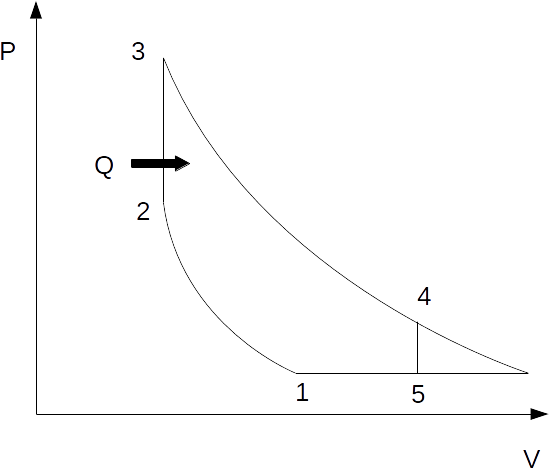
\includegraphics[width=.5\textwidth]{ThermoDiagram.png}
		\caption{PV Diagram of Modern Atkinson Cycle}
		\label{fig:diagram1}
	\end{figure}
	
	Our compression ratio is taken to be 10, a high compression ratio that prevents knocking.
	A lean air to fuel mixture ratio of 29.4 is chosen to ensure complete combustion and limit the pressures. These parameters completely define our thermal cycle.\\ Since the proportion of gasoline is small, and gasoline composed of nonpolar substances, an air standard model is used. The air is not assumed cold - the cold assumption results in far too significant of errors during the combustion process. Gas Tables are used to get air properties.
	\subsection*{Initial Constraints and Constants}
	The compression ratio and air-to-fuel ratio are listed below.
	\begin{align*}
		C_R &= \frac{V_1}{V_2} = 10 \\
		M_R &= \frac{m_A}{m_G} = 29.4
	\end{align*}
	The total volume swept by the piston is constrained by the total c.c. of the engine.
	\begin{align*}
		\frac{3000\ \text{c.c.}}{6} &= V_4-V_2 
	\end{align*}
	Point 1 and 5 are at ambient pressure $p_{amb}$, temperature $T_{amb}$, and density $\rho_{amb}$.
	\begin{align*}
		p_{amb} &= 101325\ \text{Pa} \\
		T_{amb} &= 288\ \text{K} \\
		\rho_{amb} &= 1.225\ \text{kg}\ \text{m}^{-3}
	\end{align*}
	The lower value of the heat of combustion of gasoline referenced from the U.S. EIA.
	\begin{align*}
		H_G &= 46.7\ \text{MJ}\ \text{kg}^{-1}
	\end{align*}
	\subsection*{State 1}
	This is the start of the compression stroke right after the intake stroke. The air is at ambient conditions, noted in the previous section. The specific volume is calculated and the internal energy taken from an air table.
	\begin{align*}
		u_1 &= 205.71\ \text{kJ}\ \text{kg}^{-1}\\
		v_1 &= 0.8163\ \text{m}^3\ \text{kg}^{-1}
	\end{align*}
	
	\subsection*{State 1-2}
	The process from state 1 to state 2 is adiabatic compression. The adiabatic compression is assumed isentropic. The compression ratio dictates the final specific volume.
	\begin{align*}
		C_R &= \frac{v_1}{v_2}\\
		v_2 &= \frac{v_1}{C_R}\\
		v_2 &= 0.08163\ \text{m}^3\ \text{kg}^{-1}\\
		\rho_2 &= 12.25\ \text{kg}\ \text{m}^{-3}
	\end{align*}
	Since it's an isentropic process, the final state can be found from the air table.
	\begin{align*}
		T_2 &= 703\ \text{K}\\
		u_2 &= 514.95\ \text{kJ}\ \text{kg}^{-1}
	\end{align*}
	\subsection*{State 2-3}
	The process from state 2 to state 3 is an isochoric process with heat added from combustion. The specific heat added is determined from the air to fuel ratio.
	\begin{align*}
		m_a &= m_G + m_A = m_G + M_R m_G \\
		Q &= m_G H_G \\
		q &= \frac{Q}{m_t} = \frac{H_G}{1 + M_R}\\
		q &= 1.5362\ \text{MJ}\ \text{kg}^{-1}
	\end{align*}
	With no work done on the gas, the final internal energy is given by adding the heat and initial internal energy.
	\begin{align*}
		u_3 &= q + u_2\\
		u_3 &= 2051.1\ \text{kJ}\ \text{kg}^{-1}
	\end{align*}
	The density is identical, since it's an isochoric process. Additional properties are now derived from the air table.
	\begin{align*}
		p_3 &= 8.187\ \text{MPa}\\
		T_3 &= 2385\ \text{K}\\
		\rho_3 &= 12.25\ \text{kg}\ \text{m}^{-3}\\
		p_{3r} &= 4443.2
	\end{align*}
	\subsection*{State 3-4}
	This is the expansion stroke - modeled as an adiabatic process. The pressure it expands to is chosen so enough power is produced.
	\begin{align*}
		p_4 &= 2.25 p_o = 227.98\ \text{kPa}\\
		p_{4r} &= 123.73
	\end{align*}
	Modeling the adiabatic process as isentropic, the relative pressure can be used to find the final properties.
	\begin{align*}
		T_4 &= 1022\ \text{K}\\
		u_4 &= 778\ \text{kJ}\ \text{kg}^{-1}\\
		\rho_4 &= 0.777\ \text{kg}\ \text{m}^{-3}
	\end{align*}
	\subsection*{Complete Cycle Properties}
	The isentropic processes have no heat transfer - $W = \Delta U$.\\
	The isobaric process has a simple work relation - $W = P \Delta V$.\\
	The specific work is derived from this:
	\begin{align*}
		w_{cyc} &= (u_3-u_4) - (u_2-u_1) - p_{amb}(v_4 - v_1) \\
		w_{cyc} &= 1038.3\ \text{kJ}\ \text{kg}^{-1}
	\end{align*}
	The total air mass per cylinder is now solved for:
	\begin{align*}
		\frac{3000\ \text{c.c.}}{6} &= m_a(v_4-v_2)\\
		m_a &= 414.81E-6\ \text{kg}
	\end{align*}
	One cycle is completed per piston for every 2 rotations. The power is given by the mass, specific work, and rotational frequency. The power is evaluated at 8000 R.P.M.
	\begin{align*}
		P &= 6 m_a w_{cyc} \frac{f}{2}\\
		P &= 172.28\ \text{kW}= 231.0\ \text{hp}\\
		\eta &= \frac{w_{cyc}}{q}= 67.6 \%
	\end{align*}
	Real world efficiencies are expected to be far lower.
	\newpage
	
	\section*{System Dynamics}
	
	\begin{wrapfigure}{R}{.23\textwidth}
		\centering
		\caption*{Crank Linkage}
		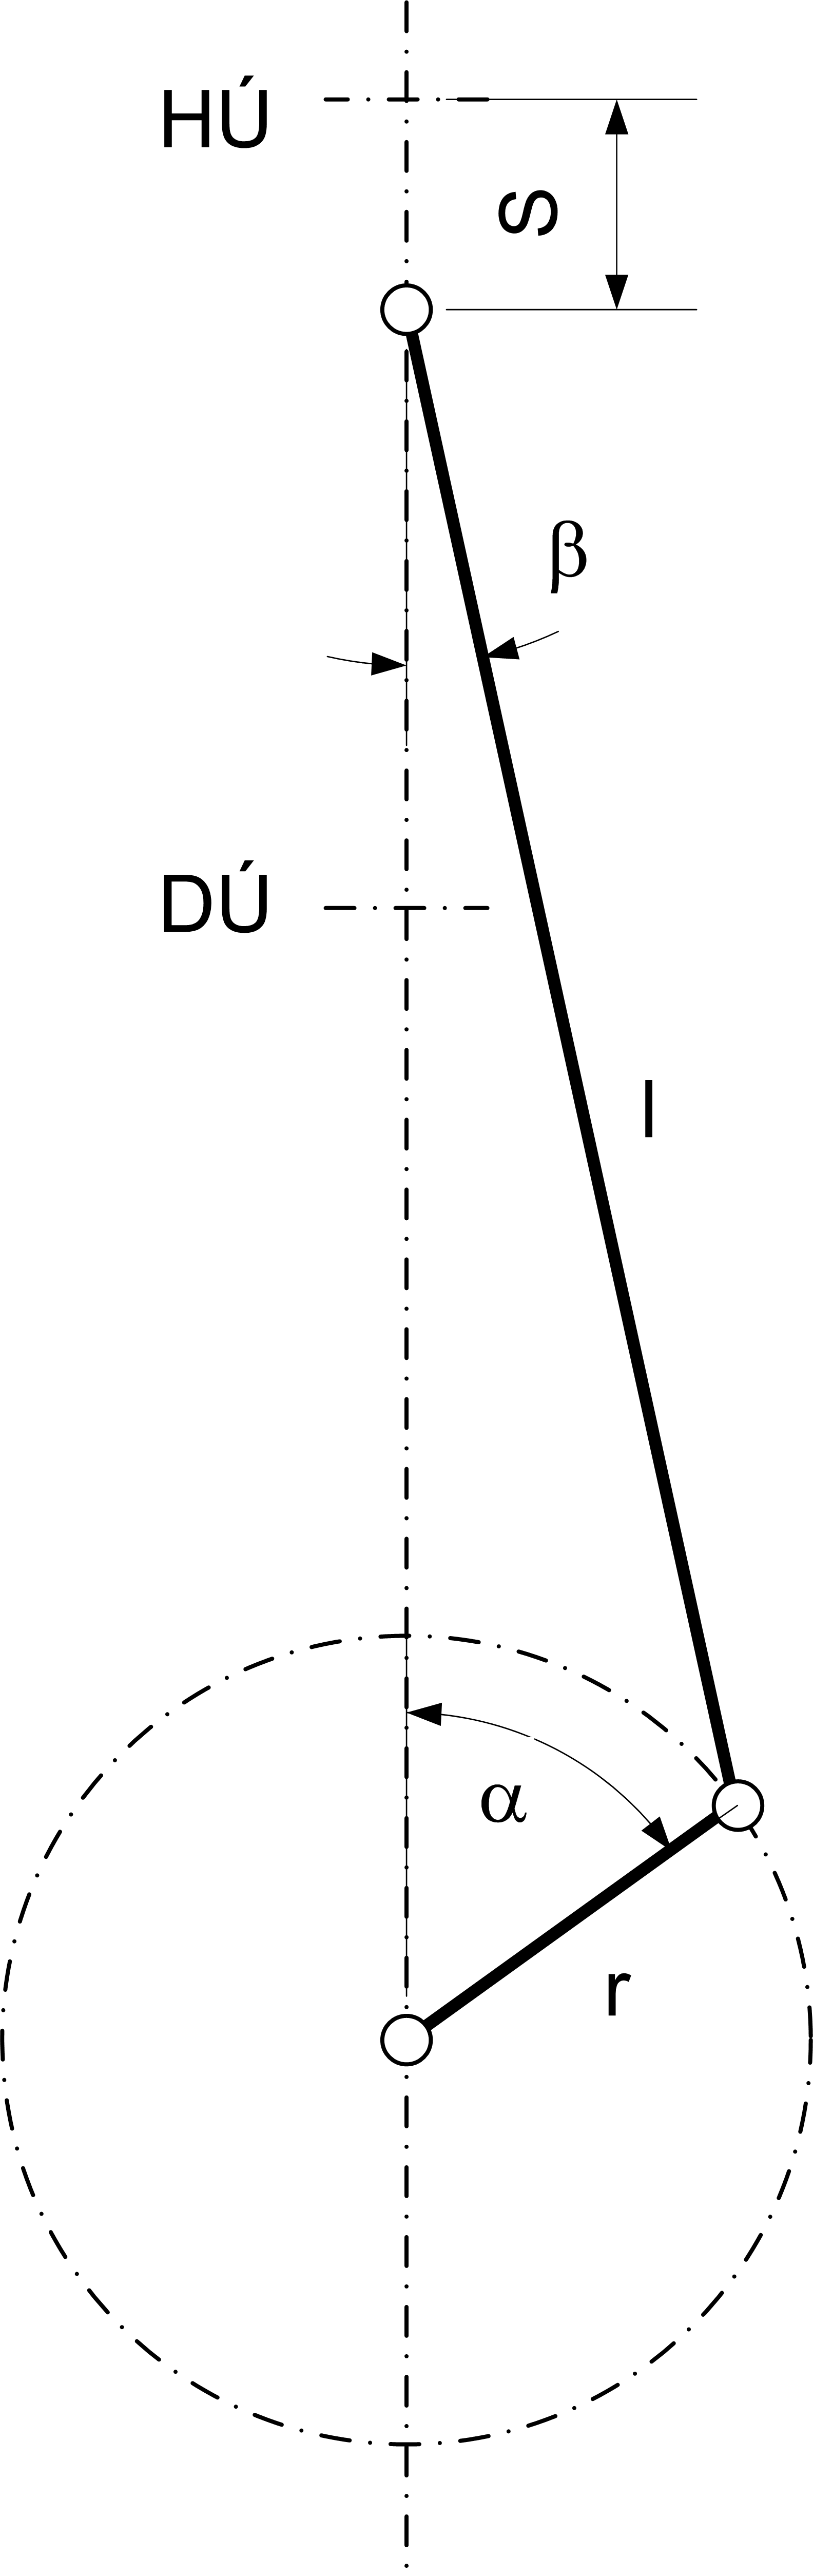
\includegraphics[width=.17\textwidth]{CrankDiagram.png}
		\label{fig:diagram2}
		\caption*{{\tiny \textit{Used with permission from WikiMedia Foundation}}}
		
	\end{wrapfigure}
	To derive the piston forces, first the linear kinematics of the piston head needs to derived with respect to $\alpha = \omega t$, where $\theta = 0$ is TDC and $x$ is the distance below TDC. \\
	The crankshaft radius is $r$ and the connecting rod length is $l_CR$. The height from the crank center is given by $r \cos (\alpha) = r \cos (\omega t)$. The height from the connecting rod is derived from noting the triangles formed by the crankshaft and connecting rod share an edge. $l_{CR} \cos (\beta)$ is solved for in terms of $\alpha$.
	\begin{align*}
		r \sin(\alpha) &= l_{CR} \sin (\beta)\\
		\frac{r}{l_{CR}}\sin(\alpha) &= \sin (\beta)\\
		\cos(\beta) &= \sqrt{1 - \Big( \frac{r}{l_{CR}}\sin(\alpha) \Big)^2}\\
		l_{CR} \cos (\beta) &= \sqrt{l_{CR}^2 - (r \sin (\alpha))^2}
	\end{align*}
	The position is given by $r \cos (\omega t) + l_{CR} \cos (\beta)$. The equation is adjusted such that $x(0)=0$ and downwards is positive. The derivatives are derived with a symbolic algebra program. These dynamic equations are used to later derive the forces on the piston and crankshaft.\\
\begin{align*}
	x(t ) &= (r + l_{CR}) - \Big(r \cos (\omega t)  + \sqrt{l_{\text{CR}}^2 - r^2 \sin^2 (\omega t )} \Big)\\
	v(t ) &=  \frac{\omega r^{2} \sin{\left (\omega t \right )} \cos{\left (\omega t \right )}}{\sqrt{l_{CR}^{2} - r^{2} \sin^{2}{\left (\omega t \right )}}} + \omega r \sin{\left (\omega t \right )}\\
	a (t) &=  \frac{\omega^{2} r^{4} \sin^{2}{\left (\omega t \right )} \cos^{2}{\left (\omega t \right )}}{\left(l_{CR}^{2} - r^{2} \sin^{2}{\left (\omega t \right )}\right)^{\frac{3}{2}}} - \frac{\omega^{2} r^{2} \sin^{2}{\left (\omega t \right )}}{\sqrt{l_{CR}^{2} - r^{2} \sin^{2}{\left (\omega t \right )}}}\nonumber \\
	&  \qquad \qquad + \frac{\omega^{2} r^{2} \cos^{2}{\left (\omega t \right )}}{\sqrt{l_{CR}^{2} - r^{2} \sin^{2}{\left (\omega t \right )}}} + \omega^{2} r \cos{\left (\omega t \right )}
\end{align*}
\begin{figure}[H]
		\centering
		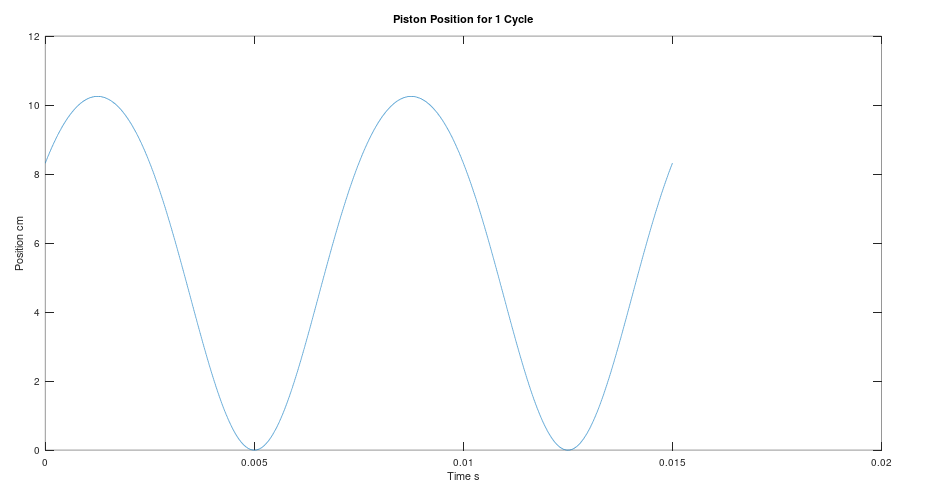
\includegraphics[width=\textwidth]{Selection_364.png}
	\end{figure}
	\begin{figure}[H]
		\centering
		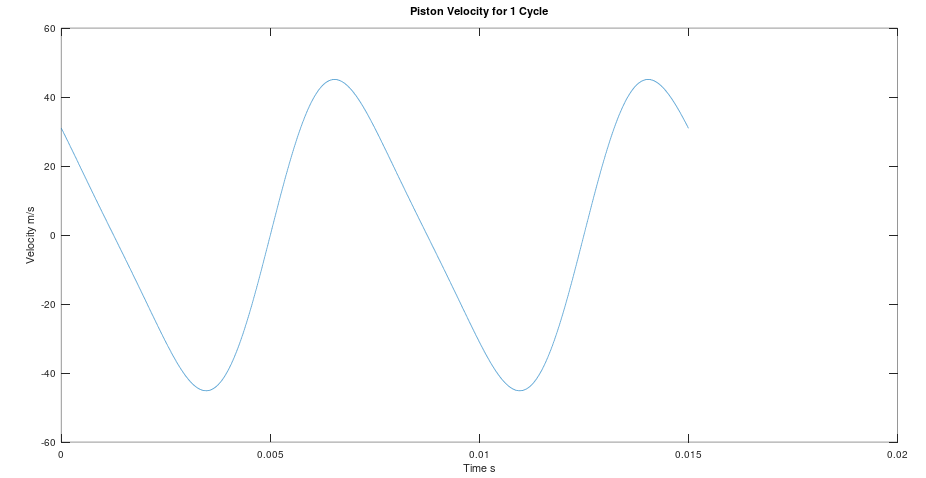
\includegraphics[width=\textwidth]{Selection_363.png}
	\end{figure}
	\begin{figure}[H]
		\centering
		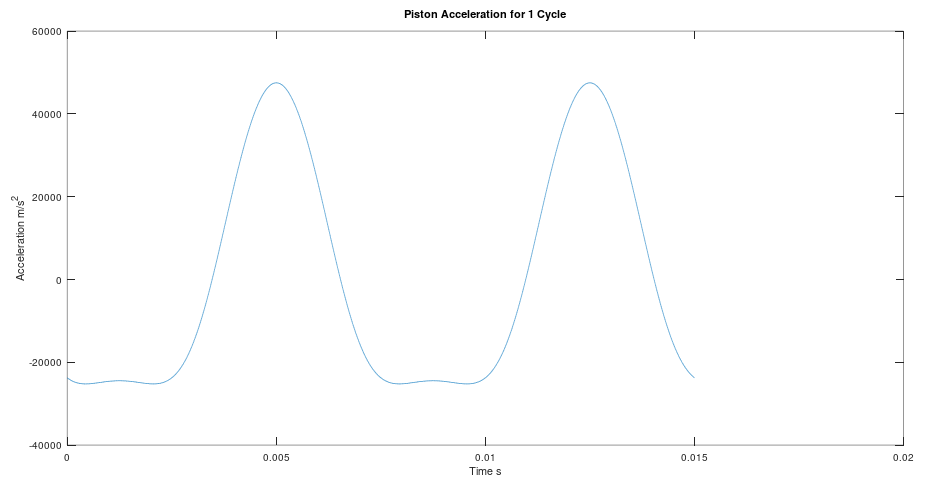
\includegraphics[width=\textwidth]{Selection_362.png}
	\end{figure}
\newpage

\section*{Forces}
To get the force of the piston, pressures equations are needed. The pressure of the expansion and compression strokes relative to piston position are approximated with the adiabatic relation $P V^{\gamma} = c$.
The pressure of the intake and compression strokes are derived using mass flow rates and Bernoulli's equation.\\
At the TDC, the height of the air column is given by $z = \frac{V_{\text{comp}}}{A_C}$, where $A_C$ is the cross sectional area of the chamber and $V_{\text{comp}}$ is the air volume at compression.\\ Thus air volume at any point of piston movement is $V(t) = A_C (x(t)+z)$.
\subsection*{Compression Stroke}
The compression stroke is derived using adiabatic relations $P V^{\gamma} = c$.
\begin{align*}
	P_{\text{amb}} V_1^{\gamma} &= P(t) V(t)^{\gamma}\\
	P_{\text{Compression}}(t) &= P_{\text{amb}} \Big( \frac{V_1}{A_C (x(t)+z)} \Big)^{\gamma}
\end{align*}
\subsection*{Expansion Stroke} 
The expansion stroke is derived the same way.
\begin{align*}
	P_{4} V_{\text{comp}}^{\gamma} &= P(t) V(t)^{\gamma}\\
	P_{\text{Expansion}}(t) &= P_{4} \Big( \frac{V_{\text{comp}}}{A_C (x(t)+z)} \Big)^{\gamma}
\end{align*}
\subsection*{Intake/Exhaust Strokes}
The pressure difference in the intake/exhaust strokes is derived using bernoulli equations. A 0 air velocity in the piston chamber is assumed. For simplicity, the density is assumed constant. The pressure difference needed to balance the air flow rates is found. \\ Let $A_I$ be the cross sectional area of the intake valve.
\begin{align*}
	Q &= A_I v_a \rho_{\text{amb}} = A_C v(t)\rho_{\text{amb}}\\
	v &= \frac{A_C v(t)}{A_I}\\
	\Delta P &= \frac{1}{2} \rho_{\text{amb}} v^2 \\
	\Delta P &= \frac{1}{2} \rho_{\text{amb}} \Big( \frac{A_C v(t)}{A_I} \Big)^2
\end{align*}
\subsection*{Gas Forces}
The force on the piston from the gasses is a function of pressure and chamber area. Compressive forces are taken to be positive. \\
 Simply, $$F_{\text{Gasses}} = A_C (P(t) - P_{\text{amb}})$$\\
 The total gas force function is given by a piecewise function. Let $\theta_c$ is the angle such that $x(t) = 9z$ and $v(t) < 0$. Then  $F_{\text{Gas}}$ is
\begin{align*}
F_{\text{Gas}}(t) &=
\begin{cases}
A_C \Big(P_{4} \Big( \frac{V_4}{A_C (x(t)+z)} \Big)^{\gamma} - P_{\text{amb}}\Big)  & 0^\circ \leq \omega t \mod 720^\circ \leq 180^\circ \\
A_C \frac{1}{2} \rho_{\text{amb}} \Big( \frac{A_C v(t)}{A_I} \Big)^2  & 180^\circ < \omega t \mod 720^\circ \leq 360^\circ \\
- A_C \frac{1}{2} \rho_{\text{amb}} \Big( \frac{A_C v(t)}{A_I} \Big)^2  & 360^\circ < \omega t \mod 720^\circ \leq 540^\circ \\
A_C \frac{1}{2} \rho_{\text{amb}} \Big( \frac{A_C v(t)}{A_I} \Big)^2 & 540^\circ < \omega t \mod 720^\circ \leq 360^\circ + \theta_c \\
A_C \Big( P_{\text{amb}} \Big( \frac{V_1}{A_C (x(t)+z)} \Big)^{\gamma}- P_{\text{amb}}\Big)  & 360^\circ + \theta_c < \omega t \mod 720^\circ < 720^\circ \\
\end{cases}
\end{align*}
\begin{figure}[H]
		\centering
		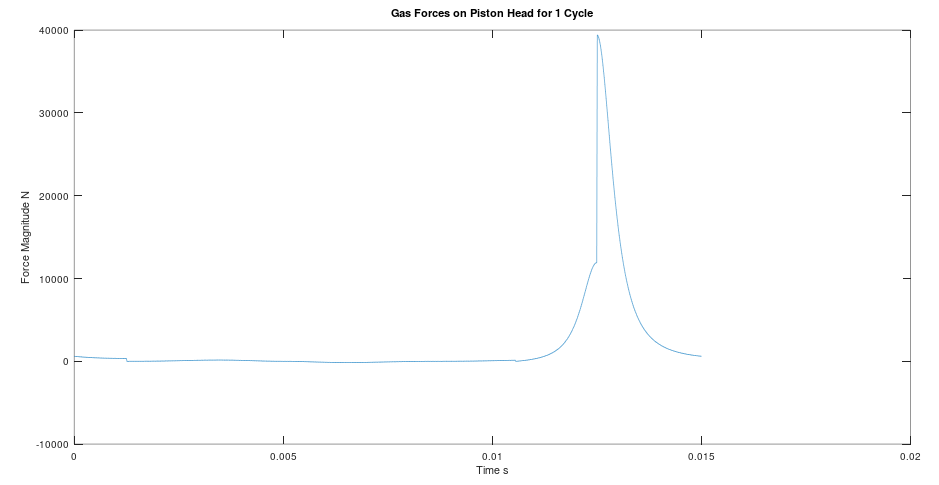
\includegraphics[width=\textwidth]{Selection_361.png}
	\end{figure}
\subsection*{Acceleration Forces}
Additionally there exists a body force present due to the acceleration of the piston head. Since compressive forces are positive, the acceleration term is inverted. Assuming $l_{CR} >> r$, the acceleration of the connecting rod is assumed equivalent to piston acceleration. For the forces on the piston, only the piston mass matters. For the forces on the crankshaft, both the piston mass $m_p$ and connecting rod mass $m_{CR}$ are needed.
$$F_{\text{Accel}}(t) = - m_p a(t)$$
The total force on the piston is from both the acceleration terms and gas force terms is added together.
Since the connecting rod is a two body force, the forces acting on the piston and crank shaft are parallel to the connecting rod. Since the vertical force is determined by the gas and acceleration, the horizontal force is determined by the angle of the connecting rod. 
\begin{align*}
	F(t) &= F_{\text{Gas}}(t)+	F_{\text{Accel}}(t)\\
	F_H &= F(t) \tan( \beta) = F(t) \frac{\sin (\beta)}{\cos (\beta)}\\
	F_H &= F(t) \frac{r \sin (\omega t)}{\sqrt{l^2 - r^2 \sin^2(\omega t)}}
\end{align*}
Finally the forcing function is given in terms of a vector equation. $\hat{i}$ is oriented upwards towards the piston and $\hat{k}$ parallel to the shaft, towards the torque output.  
\begin{align*}
\vec{F}(t) &= \big \langle -F(t)\ \hat{i},\ F(t) \frac{r \sin(\omega t)}{\sqrt{l^2 - r^2 \sin^2(\omega t)}}  \hat{j} \big \rangle
\end{align*}
\begin{figure}[H]
		\centering
		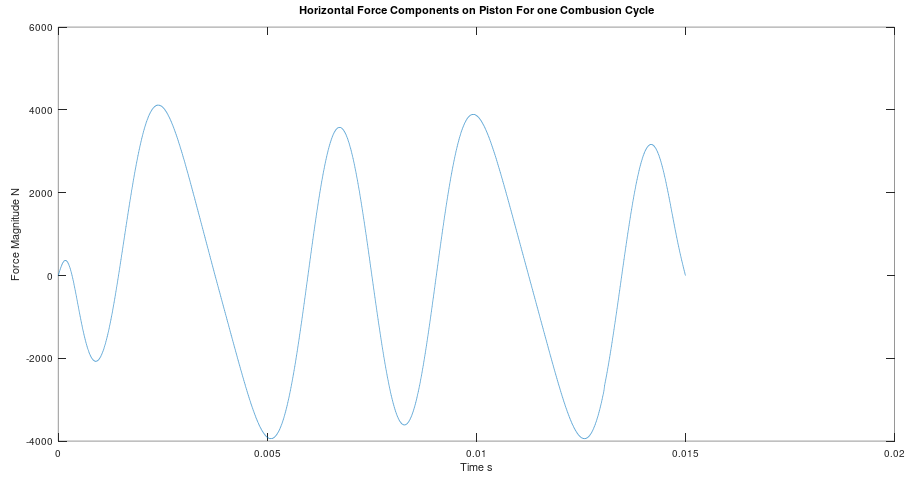
\includegraphics[width=\textwidth]{Selection_360.png}
	\end{figure}
	\begin{figure}[H]
		\centering
		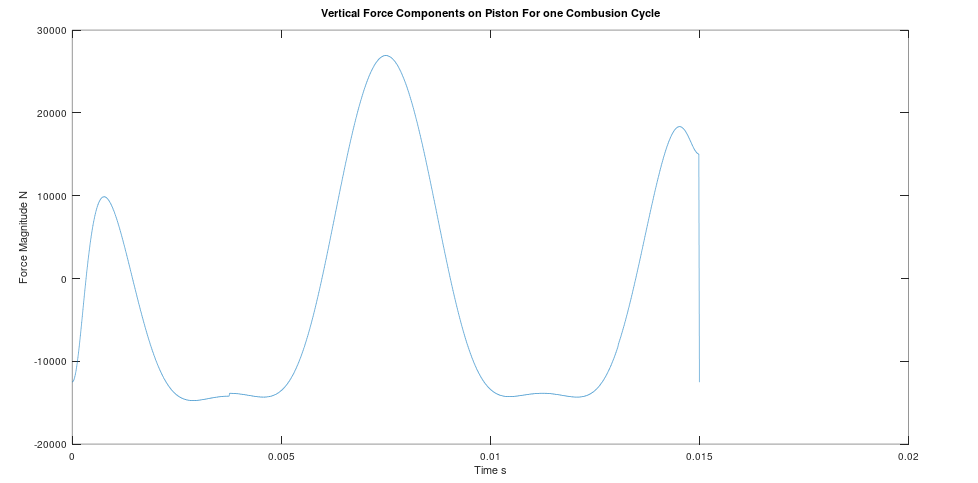
\includegraphics[width=\textwidth]{Selection_359.png}
	\end{figure}
	\begin{figure}[H]
		\centering
		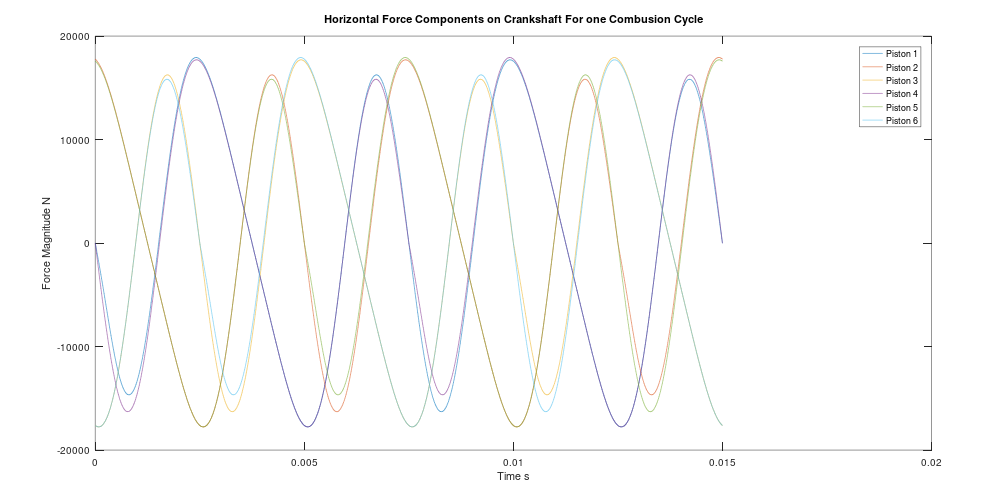
\includegraphics[width=\textwidth]{Selection_358.png}
	\end{figure}
	\begin{figure}[H]
		\centering
		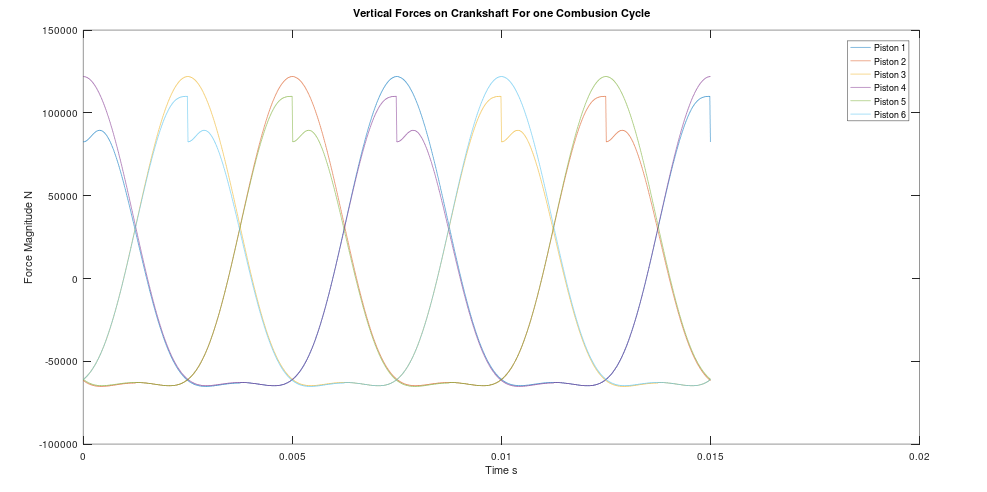
\includegraphics[width=\textwidth]{Selection_357.png}
	\end{figure}
\newpage
\section*{Piston Analysis}
The first part of the design is the design of the piston head. The piston head determines the forces acting on the rest of the body.
\subsection*{Piston Material}
The piston head is moving at high frequencies and exposed to high-temperature environments. The piston material needs to be light, creep resistant, and possess a fatigue limit to ensure a long piston head life. Stainless steels were too heavy, resulting in high forces on all parts of the assembly. Titanium Ti-6Al-4V was chosen instead, both for longevity and weight reduction. Let $E$ be the material stiffness, $S_y$ be the yield strength, $S_{eN}$ be the notched fatigue limit, $S_{\tau}$ be the shear strength, and $\rho$ be the density. 
\begin{align*}
	E_P &= 113.8\ \text{GPa}\nonumber \\
	S_{y P} &= 880\ \text{MPa}\nonumber \\
	S_{eN P} &= 240\ \text{MPa}\nonumber \\
	S_{\tau} &= 550\ \text{MPa}\nonumber \\
	\rho_P &= 4.43\ \text{g}\text{cm}^{-3}\nonumber 
\end{align*}
\subsection*{Piston Ring Material}
The piston rings need to make a simple seal between the piston head and the wall. Ductile iron is chosen, for its costs, fatigue limit, and relative softness. The particular grade is 65-45-12. The grade properties are tabulated below.
\begin{align*}
	E_R &= 168\ \text{GPa}\nonumber \\
	\nu_R &= .29\nonumber \\
	S_{y R} &= 332\ \text{MPa}\nonumber \\
	S_{eN R}&= 117\ \text{MPa}\nonumber \\ 
	\rho_R &= 7.15\ \text{g}\text{cm}^{-3}\nonumber 
\end{align*}
\subsection*{Piston \& Ring Geometry}
The piston is simply modeled as two cylinders, with the larger head on top of the tail. Two rings are located neat the top and bottom of the piston head. The tail contains a through hole for the for the connecting rod.
\begin{table}[H]
\begin{tabular}{lllll}
$d_c$ & Diameter of the Piston Chamber & 7.88 cm  \\
 $d_h$& Diameter of the Piston Head & 7.48 cm   \\
 $d_t$& Diameter of the Piston Tail & 4 cm   \\
 $d_j$& Diameter of the Joint Hole & 1.5 cm   \\
 $h_h$& Height of the Head &  6.5 cm  \\
 $h_r$& Height of the Ring &  5 mm  \\
$h_t$ & Height of the Tail &  2 cm  \\
$s_P$& Distance Swept by Piston & 10.25 cm   \\
$z_{G_1}$& Vertical Distance from Piston Top to Top Ring &  1.5 cm  \\
$z_{G_2}$& Vertical Distance from Piston Top to Bottom Ring &  5 cm  \\
$d_{Ro}$& Outer Ring Diameter &  7.89 cm  \\
$d_{Ri}$ & Inner Ring Diameter & 6.48 cm 
\end{tabular}
\end{table}
The swept distance is calculated from total piston volume. Let $A_C$ be the chamber area.
$$s_P = \frac{3000\ \text{c. c.}}{6 A_C}$$
\subsection*{Piston Ring Forces}
	\begin{figure}[h]
		\centering
		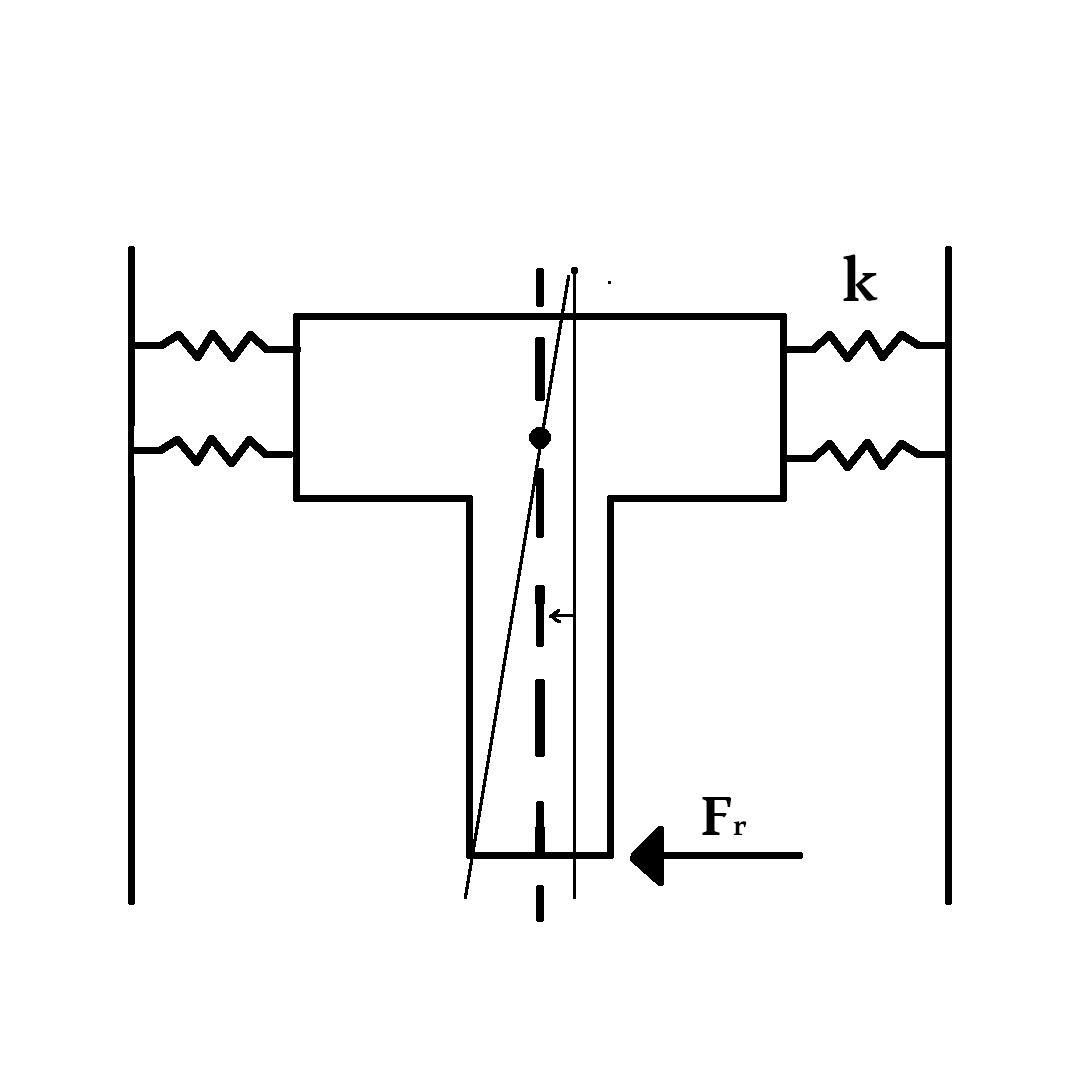
\includegraphics[width=.75\textwidth]{PistonDiagram.png}
		\caption{Ideal Gasket Forces}
		\label{fig:diagram1}
	\end{figure}
	The rings only have horizontal reactions - so only the horizontal forces are considered.
	The rings are simply modeled as springs connecting the piston to either side of the wall. Since the rings must maintain connection to the piston chamber wall, small deflections and angles are assumed. Thus small angle approximations are made.\\ Let $\theta$ be the angle the piston is rotated with respect to the vertical and $x$ the displacement of the piston.\\
	First, the center of mass of the piston is calculated. Let $V_h$ be the volume of the piston head and $V_t$ be the volume of the piston tail.
	\begin{align*}
		z_{CG} &= \frac{\frac{h_h}{2} V_h + (h_h+ \frac{h_t}{2}) V_t}{V_H + V_t} = \frac{\frac{h_h}{2}d_h^2 h_h + (h_h+ \frac{h_t}{2}) d_t^2 h_t}{d_h^2 h_h + d_t^2 h_t }
	\end{align*}
	
	The spring equations for the ring forces are written out. Let $R_{11}$ designate the upper left reaction and $R_{12}$ the upper right reaction.
	\begin{align*}
		F_{R_{11}} &= k(x - (z_{CG}-z_{G_1}) \theta) \\
		F_{R_{12}} &= k(-x + (z_{CG}-z_{G_1}) \theta) \\
		F_{R_{21}} &= k(x - (z_{CG}-z_{G_2}) \theta) \\
		F_{R_{22}} &= k(-x + (z_{CG}-z_{G_2}) \theta) 
	\end{align*}
	The moment and force equations are written out.
	\begin{align*}
		F_r &= - F_{R_{11}} + F_{R_{12}} - F_{R_{21}} + F_{R_{22}}\\
		0 &= F_r (h_h + h_t - z_{CG}) + (F_{R_{12}} - F_{R_{11}})(z_{G_1} - z_{CG})+ (F_{R_{22}} - F_{R_{21}})(z_{G_2} - z_{CG})
	\end{align*}
	Finally, x and theta are solved for.
	\begin{align*}
	\alpha &= 2 h_{h} z_{CG} - h_{h} z_{G_1} - h_{h} z_{G_2} + 2 h_{t} z_{CG} - h_{t} z_{G_1} - h_{t} z_{G_2}\\
	\beta &= - 4 z_{CG}^{2} + 3 z_{CG} z_{G_1} + 3 z_{CG} z_{G_2} - z_{G_1}^{2} - z_{G_2}^{2}\\
		x &= \frac{F_{r} \left(\alpha +\beta\right)}{2 k \left(z_{G_1}^{2} - 2 z_{G_1} z_{G_2} + z_{G_2}^{2}\right)}\\
		\theta &= \frac{F_{r} \left(2 h_{h} + 2 h_{t} - 4 z_{CG} + z_{G_1} + z_{G_2}\right)}{2 k \left(z_{G_1}^{2} - 2 z_{G_1} z_{G_2} + z_{G_2}^{2}\right)}
	\end{align*}
	The spring constant of the rings is derived in terms of material and geometric properties. To simplify calculation, the ring will be treated as a flat area cross section, assumed to fit the chamber diameter.
	\begin{align*}
		\epsilon &= \frac{\sigma}{E}\\
		\Delta t &= t \epsilon = \frac{Pt}{A_C E} \\
		A_C &= d_{c} h_g \\
		k &= \frac{P}{\Delta t} = \frac{d_{c} h_r E}{\Delta t}
	\end{align*}
	The maximum $F_r$ is calculated from the earlier force equations. The results are tabulated below.
\begin{table}[H]
\begin{tabular}{lllll}
 $F_r$ & 4.12 kN \\
 $k$& 9.46 GN $\text{m}^{-1}$  \\
 max($F_{R_{XX}}$)&  4.97 kN \\
 max($F_{R_{XX}}$)&  -4.97 kN
\end{tabular}
\end{table}
	\subsection*{Ring Stresses and Pressures}
	The average pressure difference from the reaction forces is given below:
	\begin{align*}
	 \Delta p_{G_X \text{avg}} &= \frac{F_{G_X}}{d_{ro} h_r}
	\end{align*}
	The minimum pressure which the rings must be fitted to is determined by the maximum pressure of the air $p_{AM}$ and the negative change on pressure from the piston forces. This ensures the piston rings are greater than $p_{AM}$ at all parts of the cycle.
	\begin{align*}
	p_{\text{fit}} &\geq p_{AM} - \frac{\text{min} \{ F_{G_X}, 0 \}}{d_{ro} h_r} = 20.8\ \text{MPa}\\
	p_{\text{fit}} &= \frac{\Delta}{\frac{D_{hi}}{E_h} \Big( \frac{D_{ho}^2+D_{hi}^2}{D_{ho}^2-D_{hi}^2} + \nu_h \big) +\frac{D_{so}}{E_h} \Big( \frac{D_{so}^2+D_{si}^2}{D_{so}^2-D_{si}^2} + \nu_s \big) } = 63.7\ \text{MPa}
	\end{align*}
	The radial ring stress is simply the pressure on the ring. Since the ring is thin walled, a constant radial stress is assumed.
	Since the rings are supported by the piston head, the tangential stress is derived using a thick walled pressure vessel equation, with a solid pressure vessel. Since the inner radius is 0, the resulting stresses are identical.
	\begin{align*}
		\sigma_{r r} &= -p\\
		\sigma_{r t} &= -p
	\end{align*}
	The pressures also attempts to push out the ring. The push out stress is derived below. The shear force $V$ is given by the pressure acting on the area of the ring directly exposed to the chamber.
	\begin{align*}
	 V &= \frac{\pi}{4}(d_{c}^2-d_{h}^2) p\\
	 \tau_{\text{max}} &= \frac{3V}{2A} \\
	 \tau_{rp} &= \frac{3V}{2 h_r \pi \frac{d_h}{2} } = \frac{3 \pi (d_{c}^2-d_{h}^2) p}{4 h_r \pi d_h} 
	\end{align*}
	Finally, friction creates a shear force on the ring. Since the ring reactions are equal and opposite, $p_{\text{avg}} = p_{\text{fit}}$.
	\begin{align*}
		V &=  \mu p_{\text{avg}} A_o \\
		\tau_{\text{max}} &= \frac{3V}{2A_h} \\
		\tau_{f} &= \frac{3 \mu p_{\text{fit}} d_{go}^2}{d_h^2} 
	\end{align*}
	The minimum and maximum of each ring stress is tabulated. Since the rings are fitted to compression, 
	\begin{align*}
		\sigma_{r r\ \text{min}} &= \sigma_{rt\ \text{min}} = p_{\text{fit}} + \frac{\text{min} \{ F_{G_X}, 0 \}}{d_{go} h_g}\\
		\sigma_{rr\ \text{max}} &= \sigma_{rt\ \text{max}} = p_{\text{fit}} + \frac{\text{max} \{ F_{G_X}\}}{d_{go} h_g}\\
		\tau_{r\ \text{max}} &= \frac{3  (d_{go}^2-d_{h}^2) p_{AM}}{4 h_g d_h} + \frac{3 \mu p_{\text{fit}} d_{go}^2}{d_h^2}\\
		\tau_{r\  \text{min}} &= -\frac{3 \mu p_{\text{fit}} d_{go}^2}{d_h^2}
	\end{align*}
	The resulting stresses and the maximum Von Mises stress and associated factor of safety is calculated.
\begin{table}[H]
\begin{tabular}{lllll}
 $\sigma_{r r\ \text{max}}$ & 76.3 MPa \\
 $\sigma_{r r\ \text{min}}$& 51.0 MPa \\
 $\sigma_{t r\ \text{max}}$ & 76.3 MPa \\
 $\sigma_{t r\ \text{min}}$& 51.0 MPa \\
 $\tau_{r\ \text{max}}$ &  20.7 MPa \\
 $\tau_{r\  \text{min}}$&  -10.6 MPa \\
 $\sigma'_{\text{max}}$ & 84.3 MPa\\
 Factor of Safety & 3.9
\end{tabular}
\end{table}
The amplitude and mean stresses are tabulated for fatigue analysis. 
$$\sigma'_a = \sqrt{\frac{1}{2} \big( \frac{\sigma_{rr a}}{.85} \big)^2 + \frac{1}{2} \big( \frac{\sigma_{rt a}}{.85} \big)^2 + 3 \tau_{r a}^2}$$
$$\sigma'_m = \sqrt{\frac{1}{2} \sigma_{rr m}^2 + \frac{1}{2} \sigma_{rt m}^2 + 3 \tau_{r a}^2}$$
The factor of safety is given by the modified Goodman equation:
$$\frac{\sigma_a}{S_{eN}} + \frac{\sigma_m}{S_{ut}} = \frac{1}{n} $$

\begin{table}[H]
\begin{tabular}{lllll}
 $\sigma_{r r a}$ & 25.2 MPa \\
 $\sigma_{r t a}$& 25.2 MPa \\
 $\tau_{r a}$&  15.7 MPa \\
 $\sigma_{r r m}$ & 63.7 MPa \\
 $\sigma_{r t m}$& 63.7 MPa \\
 $\tau_{r m}$&  5.1 MPa \\
 $\sigma'_{a}$ & 58.8 MPa\\
 $\sigma'_{m}$ & 64.3 MPa\\
 Factor of Safety & 1.56
\end{tabular}
\end{table}
Since the factor of safety is greater than 1 using the notched fatigue limit, the piston rings are expected to have a long life.
	\subsection*{Axial Piston Stress Calculations}
	The axial force on the head is determined by the maximum force on the piston $F_M$. The loading cycle can be roughly approximated from $F_M$ to $-F_M$. Due to the pistons extremely short length, horizontal forces are ignored for deflection and moment. The resultant stress from the from the pressure in the piston major diameter is given below.
	\begin{align*}
		\sigma_{z\ \text{Head}} &= - \frac{4 F_M}{\pi d_h^2}
	\end{align*}
	In the ring channels, a greater compression stress results from the smaller diameter and push out forces on the ring. The channels also experience radial stresses from the rings. Stress concentration factors $K = 3.5$ are added due to the geometry of the channel.
	\begin{align*}
		\sigma_{z\ \text{Force}} &=  K \sigma_{z\ \text{Head}} \frac{d_h^2}{d_{ri}^2} \\
		\sigma_{z\ \text{Push Out}} &= - K p \frac{d_{c}^2 - d_h^2}{d_h^2 - d_{ri}^2}\\
		\sigma_{z\ \text{Channel}} &= K \sigma_{z\ \text{Head}} \frac{d_h^2}{d_{ri}^2} - K p \frac{d_{ro}^2 - d_h^2}{d_h^2 - d_{gi}^2}\\
		\sigma_{r\ \text{Channel}} &= \sigma_{r r}
	\end{align*}
	The tail of the piston also has a concentration factor due to the diameter change, represented by $K_2 = 1.5$. The tail experiences different stresses when in tension. Let $A_c$ be the area of the smallest chord formed by joint hole and piston tail.
	\begin{align*}
		\sigma_{z\ \text{Tail}} &= K_2 \sigma_{z\ \text{Head}} \frac{d_h^2}{d_t^2}\\
		\sigma_{z\ \text{Joint Compression}} &= \sigma_{z\ \text{Head}} \frac{\pi d_h^2}{4 (\pi d_h^2/4-2*A_c)}\\
		\sigma_{z\ \text{Joint Tension}} &= -\sigma_{z\ \text{Head}} \frac{\pi d_h^2}{4 A_c}
	\end{align*}
	Finally, a push out shear is present due to the joint. An upper limit is given by distributing the shear force among the chord area from the joint hold and piston tail.
	\begin{align*}
		V &= \frac{F_R}{2}\\
		\tau &\leq \frac{3 F_R}{4 A_c}
	\end{align*}
	The vertical deflection is estimated using $\delta = L \frac{\sigma}{E}$.
	\begin{align*}
		\delta_{\text{Head}} &= - \frac{l_h p}{E}\\ 
		\delta_{\text{Tail}} &= - \frac{l_t p \frac{d_h^2}{d_t^2}}{E}\\ 
		\delta_{\text{Total}} &=  \frac{l_h p -l_t p \frac{d_h^2}{d_t^2}}{E}
	\end{align*}
	The piston forces and stresses are tabulated.
\begin{table}[H]
\begin{tabular}{lllll}
 $F_M$ & 26.9 kN \\
 $\sigma_{z\ \text{Head}}$& -6.13 MPa \\
 $\sigma_{r \text{Channel}}$ & 76.3 MPa \\
 $\sigma_{z\ \text{Force}}$ & -12.9 MPa \\
 $\sigma_{z\ \text{Channel}}$& -28.6 MPa \\
 $\sigma'_{\text{Channel}}$ &  93.6 MPa \\
 $\sigma_{z\ \text{Tail}}$&  -32.1 MPa \\
 $\sigma_{z\ \text{Joint Compression}}$ & -45.9 MPa\\
 $\sigma_{z\ \text{Joint Tension}}$ & 40.13 MPa\\
 $\tau$ & 9.2 MPa\\
 Factor of Safety & 9.4
\end{tabular}
\end{table}
Since the force completely reverses, each of these can be taken worst case as a completely alternating axial force. With a notched fatigue strength of 240 MPa, the fatigue factor of safety is 2.2.\\
The final calculated deflection was .005 mm.
\newpage

\section*{Connecting Rod Analysis}
The connecting rod can be modeled with a rectangular cross section (BxH) and as a two-force member. The maximum internal axial reaction force is taken from the gas and acceleration forces $F_M$ = 26.9 kN.
Axial stress due to $F_M$ can be found as in Equation 2.
<Insert eqn 2>
\[{\sigma _{{x_N}}} = \frac{F_M}{{{A_c}}} = \frac{F_M}{b h}\]
The next consideration is stress caused due to the maximum inertial torque possessed by the rod. That can be determined using the mass moment of inertia about the pivot point and maximum angular acceleration of the rod. Maximum angular acceleration occurs when the piston is at top dead center at the start of the expansion stroke. It is given by Equation 3 and the inertial torque can be found using Equation 4.
\[\mathop \theta \limits^{..} (x = 0) = \frac{1}{{b\sqrt {{L^2} - {b^2}} }}\]
\[{M_{bending,\max }} = {I_{mass}} \times {\mathop \theta \limits^{..} _{\max }} = {I_{mass}} \times \frac{1}{{b\sqrt {{L^2} - {b^2}} }}\]
An assumption that was made was the minimum angular acceleration is zero. Therefore, the minimum inertial torque would be zero as well. The axial stress caused by the inertial torque can be found using Equation 5.
\[{\sigma _{{x_{bend}}}} =  \pm \frac{{{M_{bend}}y}}{{{I_{area}}}} =  \pm \frac{{{M_{bend}}({\raise0.7ex\hbox{$H$} \!\mathord{\left/
 {\vphantom {H 2}}\right.\kern-\nulldelimiterspace}
\!\lower0.7ex\hbox{$2$}})}}{{{\raise0.7ex\hbox{$1$} \!\mathord{\left/
 {\vphantom {1 {12}}}\right.\kern-\nulldelimiterspace}
\!\lower0.7ex\hbox{${12}$}}B{H^3}}}\]
The two axial stress can then be combined by simply superimposing them. Following the sign convention, both the forces will cause compressive axial stresses and add up to give a total compressive stress. Since no other forces are taken into consideration, this total stress also becomes the von Mises stress acting in the rod as described by Equation 6.
\[{\sigma _x} = \frac{F_M}{b h} - \frac{{{M_{bend}}({\raise0.7ex\hbox{$H$} \!\mathord{\left/
 {\vphantom {H 2}}\right.\kern-\nulldelimiterspace}
\!\lower0.7ex\hbox{$2$}})}}{{{\raise0.7ex\hbox{$1$} \!\mathord{\left/
 {\vphantom {1 {12}}}\right.\kern-\nulldelimiterspace}
\!\lower0.7ex\hbox{${12}$}}B{H^3}}} = \sigma '\]
Finally, the yielding factor of safety can be determined using Equation 7.
\[n = \frac{{{S_y}}}{{\sigma '}}\]
In parallel to failure by yielding, buckling failure must also be considered. An end condition value of C equal to 1 was determined to be most appropriate for this scenario. The length condition can be evaluated as given in Equation 8.
\[L \ge \sqrt {\frac{{2{\pi ^2}EI}}{{{S_y}{A_c}}}} \]
Based on the length condition, the critical buckling force for either case can be found using Equation 9 and 10.
\[{P_{c{r_1}}} = \frac{{{\pi ^2}EI}}{{{L^2}}}\]
\[{P_{c{r_2}}} = {S_y}{A_c} - {\left( {\frac{{{S_y}L}}{{2\pi }}} \right)^2}\frac{{A_c^2}}{{EI}}\]
The buckling factor of safety can then be calculated as the ratio of the critical force and force F1 as given in Equation 11.
\[n = {P_{cr}} \times \frac{{\frac{b}{L}\sin ({{\cos }^{ - 1}}\frac{x}{b})}}{{{P_{cyl}}{A_{piston}}}}\]
Yet another consideration for the rod design is failure due to fatigue. Two approaches are used – linear elastic fracture mechanics (LEFM) and the stress life method. The former yields how many cycles the part can take before an initial crack reached critical crack size while the latter tells the factor safety associated with infinite fatigue life for the part.
As for LEFM, the maximum crack size can be found using Equation 12 where the stress intensity modification factor Beta is chosen to be 1 as a conservative estimate. Furthermore, the part can be modelled as a flat plate under axial loading with a surface crack.
\[{a_f} = \frac{1}{\pi }{\left( {\frac{{{K_{IC}}}}{{\beta \sigma '}}} \right)^2}\]
An initial crack size of 1 mm is used. The number of cycles to failure can be found using Paris law as given in Equation 13.
\[{N_f} = \frac{1}{{C{{\left( {\Delta \sigma \beta \sqrt \pi  } \right)}^m}}}\left[ {\frac{{{a^{1 - {\raise0.7ex\hbox{$m$} \!\mathord{\left/
 {\vphantom {m 2}}\right.\kern-\nulldelimiterspace}
\!\lower0.7ex\hbox{$2$}}}}}}{{1 - {\raise0.7ex\hbox{$m$} \!\mathord{\left/
 {\vphantom {m 2}}\right.\kern-\nulldelimiterspace}
\!\lower0.7ex\hbox{$2$}}}}} \right]_{{a_0}}^{{a_f}}\]
As for the stress-life method, the Soderberg criteria was used to remain conservative. No stress concentrations are taken into account as the rod is a straight uniform part. Therefore, the theoretical and fatigue stress concentration factors will be set to be unity. The axial stresses due to force F1 and inertial torque in the rod cycle between zero and their maximum values as defined in Equations 2 and 5 respectively. Therefore, the fatigue stresses can be calculated as given in Equations 14 and 15.
\[{\sigma _a}' = {\sigma _{{a_{bend}}}} + \frac{{{\sigma _{{a_N}}}}}{{0.85}}\]
\[{\sigma _m}' = {\sigma _{{m_{bend}}}} + {\sigma _{{m_N}}}\]
Equations 16 through 18 define the surface modification factors and fully corrected endurance limit.
\[{k_a} = a \times {S_{ut}}^b\]
\[{k_b} = \min \left( {0.88{{\left( {0.808\sqrt {BH} } \right)}^{ - 0.107}},0.91{{\left( {0.808\sqrt {BH} } \right)}^{ - 0.157}}} \right)\]
\[{S_e} = {k_a}{k_b}{S_e}' = {k_a}{k_b} \times \min \left( {\frac{{{S_{ut}}}}{2}kpsi,100kpsi} \right)\]
Finally, the fatigue factor of safety can be calculated using Equation 19.
\[n = {\left( {\frac{{{\sigma _a}'}}{{{S_e}}} + \frac{{{\sigma _m}'}}{{{S_y}}}} \right)^{ - 1}}\]
\newpage
\section*{Crankshaft Analysis}
\subsection*{Crankshaft Material}
The crankshaft's largest limiting factor is its stiffness. Since steels have roughly the same stiffness, a 1050 steel is chosen for its cost and accessibility.
\begin{table}[H]
\begin{tabular}{lllll}
$E_{CS}$ & 200 GPa  \\
 $\nu_{CS}$&  .29   \\
 $S_{y CS}$&  580 MPa  \\
 $S_{ut CS}$&  690 MPa  \\
 $\rho_{CS}$& 7.85 $\text{g}\text{cm}^{-3}$  
\end{tabular}
\end{table}
\subsection*{Crankshaft Dimensions}
\begin{table}[H]
\begin{tabular}{lllll}
$r_c$ & Crank Radius & 5.13 cm  \\
 $l_c$& Length of Crank Sections & 7.48 cm   \\
 $l_s$& Length of Shafts Between Cranks & 1 cm   \\
 $t_b$& Thickness of Crank Connectors & 2 cm   \\
 $l_a$& Length of each Crank \& Shaft subsection. & 12.48 cm $l_a = l_s + 2t + l_c$  \\
 $l_b$& Length of Shaft Section to Bearing Closest to Flywheel &  3 mm  \\
$l_s$ & Total Length of the Shaft Between the Two Bearings &  77.88 cm  \\
$d_s$& Shaft and Crank Diameters & 7.5 cm
\end{tabular}
\end{table}
\subsection*{Crankshaft Forces}
Both the connecting rod and piston weight have acceleration forces that are put on the crankshaft. The total vertical magnitude of the forces is given by:
$$F(t) = A_C (P(t) - P_{\text{amb}}) - (m_P+m_{CR})a(t)$$
As calculated earlier, the forces can be represented by vectors. The crankshaft has 6 pistons, each whose gas cycles are equally offset. Since the gas cycle has a period of 720\degree , the pistons cycles are each offset by 120\degree . Since each piston is offset by 120 degrees, each force equations is offset by $\omega t = \frac{2 \pi}{3}$ from the previous piston. The vector force equations for piston $n$ is given by:
\begin{align*}
\vec{F}(t) &= \big \langle -F(t)\ \hat{i},\ F(t) \frac{r \sin(\omega t)}{\sqrt{l^2 - r^2 \sin^2(\omega t)}}  \hat{j} \big \rangle\\
\vec{F}_n(t) &= \vec{F}(t + 120 \degree (n-1)\omega^{-1})
\end{align*} 

The direction of each crank shaft is offset by 120\degree\ too.
\begin{align*}
	\vec{r}_n = r_c \Big \langle \cos (\omega t + 120 \degree (n-1)  )\ \hat{i},\ \sin (\omega t + 120 \degree (n-1))\ \hat{j}  \Big \rangle
\end{align*}
For the shaft coordinates, the $\hat{k}$ vector is parallel to the axis of the shaft, from the first bearing to the second. The torque equation along the shaft is simply written out using cross products.
\begin{align*}
	\vec{T}(x) &= \sum_{n=1}^6 \langle x - l_a (n-1) - l_b - \frac{l_c}{2} - t\rangle^0\ \vec{F}_n \times \vec{r}_n 
\end{align*}
There are two reaction forces at each of the bearings, $\vec{R}_1$ and $\vec{R}_2$. The force and moment equations are written out to solve for these.
\begin{align*}
	\sum \vec{F} &= \vec{R}_1 + \vec{R}_2 + \sum_{n=1}^6 \vec{F}_n = 0 \\
	\sum \vec{M} &= \vec{R}_2 l_s \hat{j} + \sum_{n=1}^6 \vec{F}_n  ( l_s - l_a (n-1) - l_b - \frac{l_c}{2} - t)\ \hat{j} = 0\\
	\vec{R}_2 &= - \sum_{n=1}^6 \frac{\vec{F}_n ( x - l_a (n-1) - l_b - \frac{l_c}{2} - t)}{l_s}\\
	\vec{R}_1 &= -\vec{R}_2 - \sum_{n=1}^6 \vec{F}_n
\end{align*}
The shear and moment equations are derived below. The shear and moment is not affected by the crank offset, since there are no axial forces. Thus the crankshaft can be treated as a regular beam.
\begin{align*}
	\vec{V}(x) &= \vec{R}_1 \langle x \rangle^0 + \sum_{n=1}^6 \vec{F}_n\ \langle x - l_a (n-1) - l_b - \frac{l_c}{2} - t\rangle^0\\
	\vec{M}(x) &= \vec{R}_1 \langle x \rangle + \sum_{n=1}^6 \vec{F}_n\ \langle x - l_a (n-1) - l_b - \frac{l_c}{2} - t\rangle\\
	E_{CS} I (x) \vec{y'}(x) &= \frac{1}{2}\vec{R}_1 \langle x \rangle^2 + \frac{1}{2}\sum_{n=1}^6 \vec{F}_n\ \langle x - l_a (n-1) - l_b - \frac{l_c}{2} - t\rangle^2 + C_1\\
	E_{CS} I (x) \vec{y'}(x) &= \frac{1}{6}\vec{R}_1 \langle x \rangle^3 + \frac{1}{6}\sum_{n=1}^6 \vec{F}_n\ \langle x - l_a (n-1) - l_b - \frac{l_c}{2} - t\rangle^3 + C_1 x\\
\end{align*}
The maximum moment and shear stresses are given. To give an upperbound of moment stress, the crank moment of inertia is used for the entire length of the beam. The shear stress equation only applies for the on axis shafts.
\begin{align*}
	\sigma_M (x) = \pm \frac{|\vec{M}(x)| d(x)}{2 I_s}\\
	\tau (x) = \frac{|T(x)| d (x)}{2 J_s}
\end{align*}
The deflections, slope, and stresses of the shaft are given upper bounds by assuming a constant $I = \pi \frac{d_s^4}{64}$ across the shaft.
The maximum of each are tabulated. Here the fatigue limit is estimated by $S_{ut}/2$.

\begin{table}[H]
\begin{tabular}{lllll}
 $\sigma_M$ & $\pm$ 236.0 MPa \\
 $\tau$ & 99.7 MPa \\
 $\sigma'$ & 292.4 MPa \\
 Factor of Safety & 1.98 \\
 Fatigue Factor of Safety &  1.16 \\
 Maximum Slope &  .014 \\
 Maximum Deflection & 2.98 mm
\end{tabular}
\end{table}

Representative graphs of the crankshaft state are shown below.
\begin{figure}[h]
		\centering
		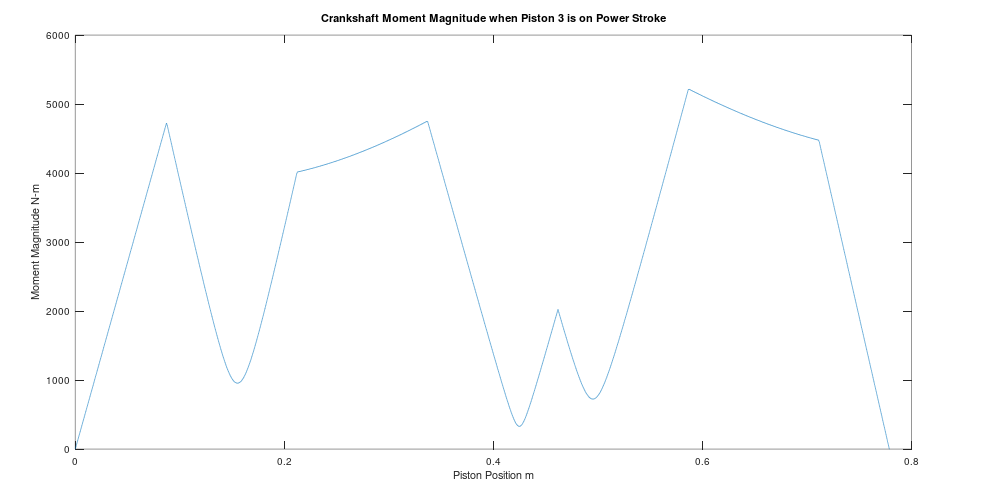
\includegraphics[width=\textwidth]{csm.png}
	\end{figure}
	\begin{figure}[h]
		\centering
		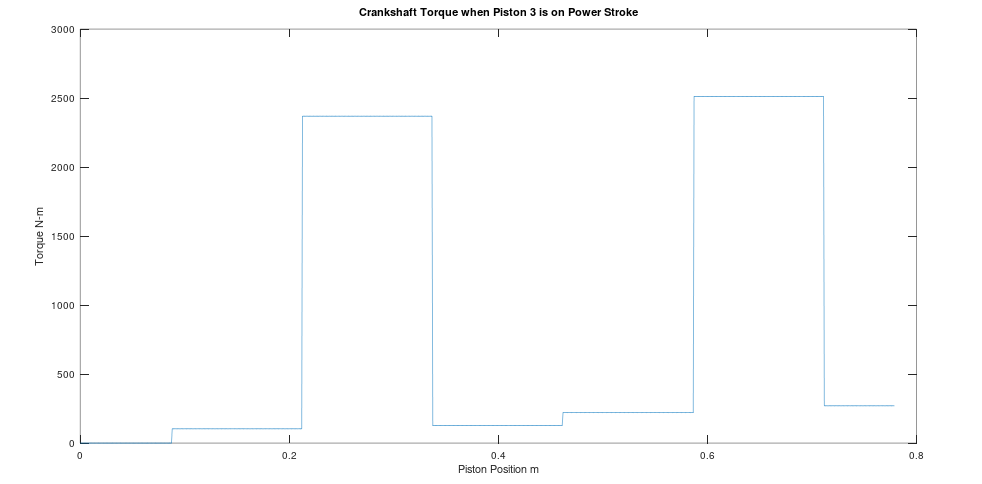
\includegraphics[width=\textwidth]{cst.png}
	\end{figure}
	\begin{figure}[h]
		\centering
		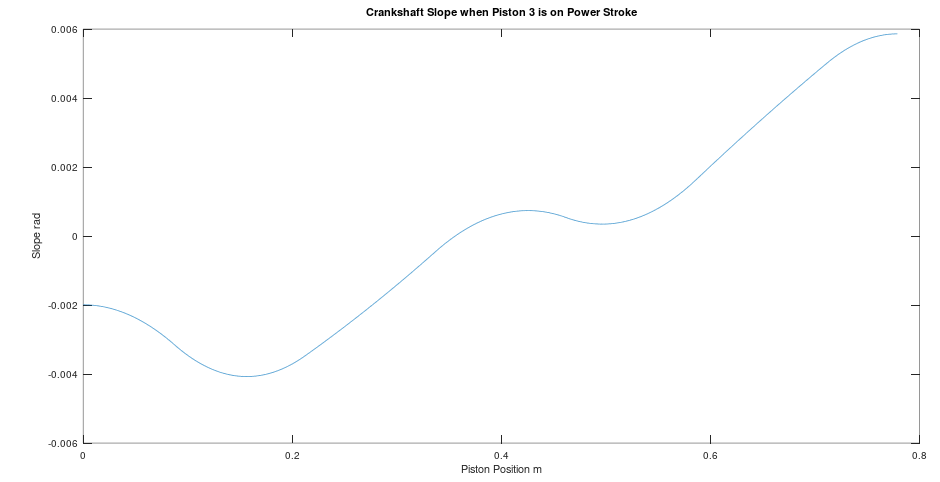
\includegraphics[width=\textwidth]{css.png}
	\end{figure}
	\begin{figure}[h]
		\centering
		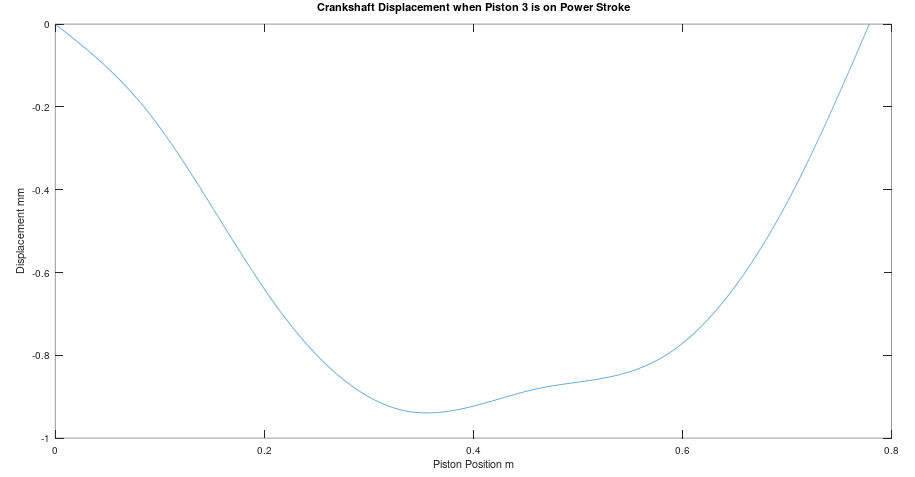
\includegraphics[width=\textwidth]{csd.png}
	\end{figure}
	\newpage
\subsection*{Flywheel Inertia}
The flywheel should have enough second moment of inertia $I_f$ to store enough energy to slow down a reasonable number of RPMs to make up the energy of a complete piston misfire. The RPMs chosen is 2000 RPM to 1000 RPM.
\newpage
\begin{align*}
	m_a w_{\text{cyc}} &= I(\omega_1^2 - \omega_2^2)\\
	I &= \frac{m_a w_{\text{cyc}}}{\frac{4 \pi^2}{60^2}(2000^2-1000^2)}\\
	I &= .0131\ \text{kg m}^2
\end{align*}
\newpage
\section*{Simulation}
\begin{figure}[h]
		\centering
		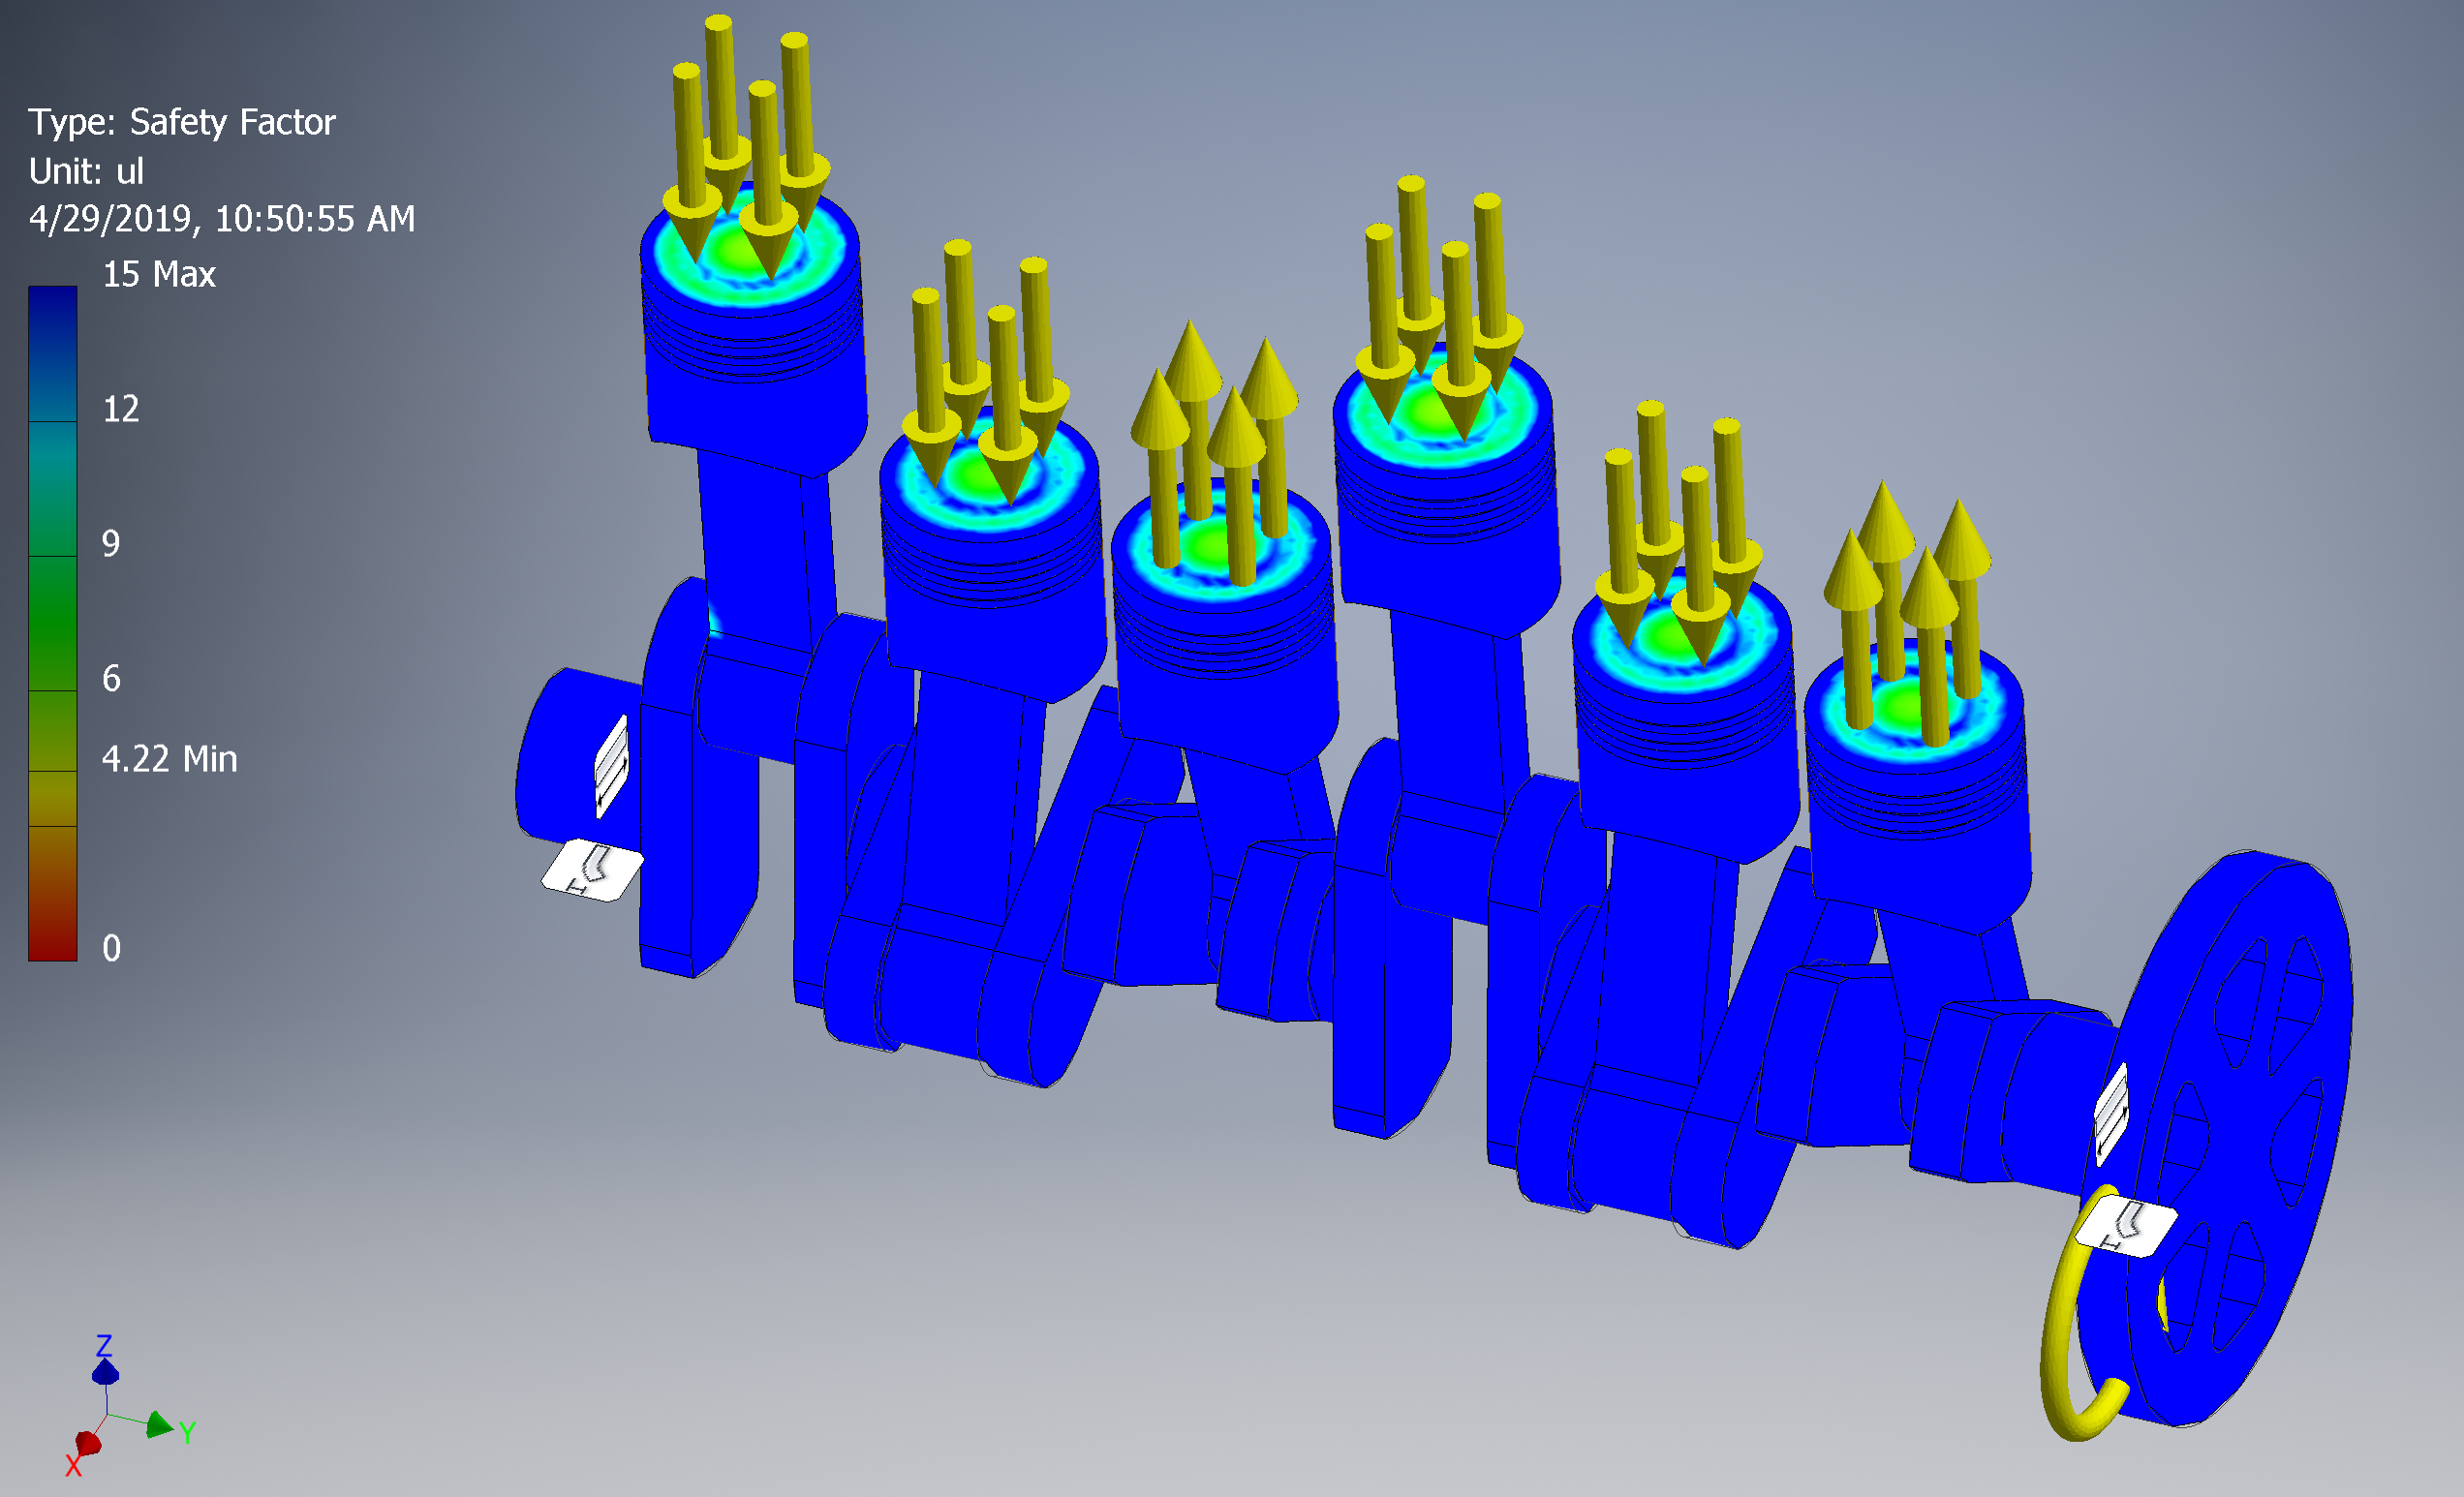
\includegraphics[width=\textwidth]{h.png}
		\caption{Factor of Safety Analysis performed in SolidWorks}
		\label{fig:diagram3}
	\end{figure}
	\begin{figure}[h]
		\centering
		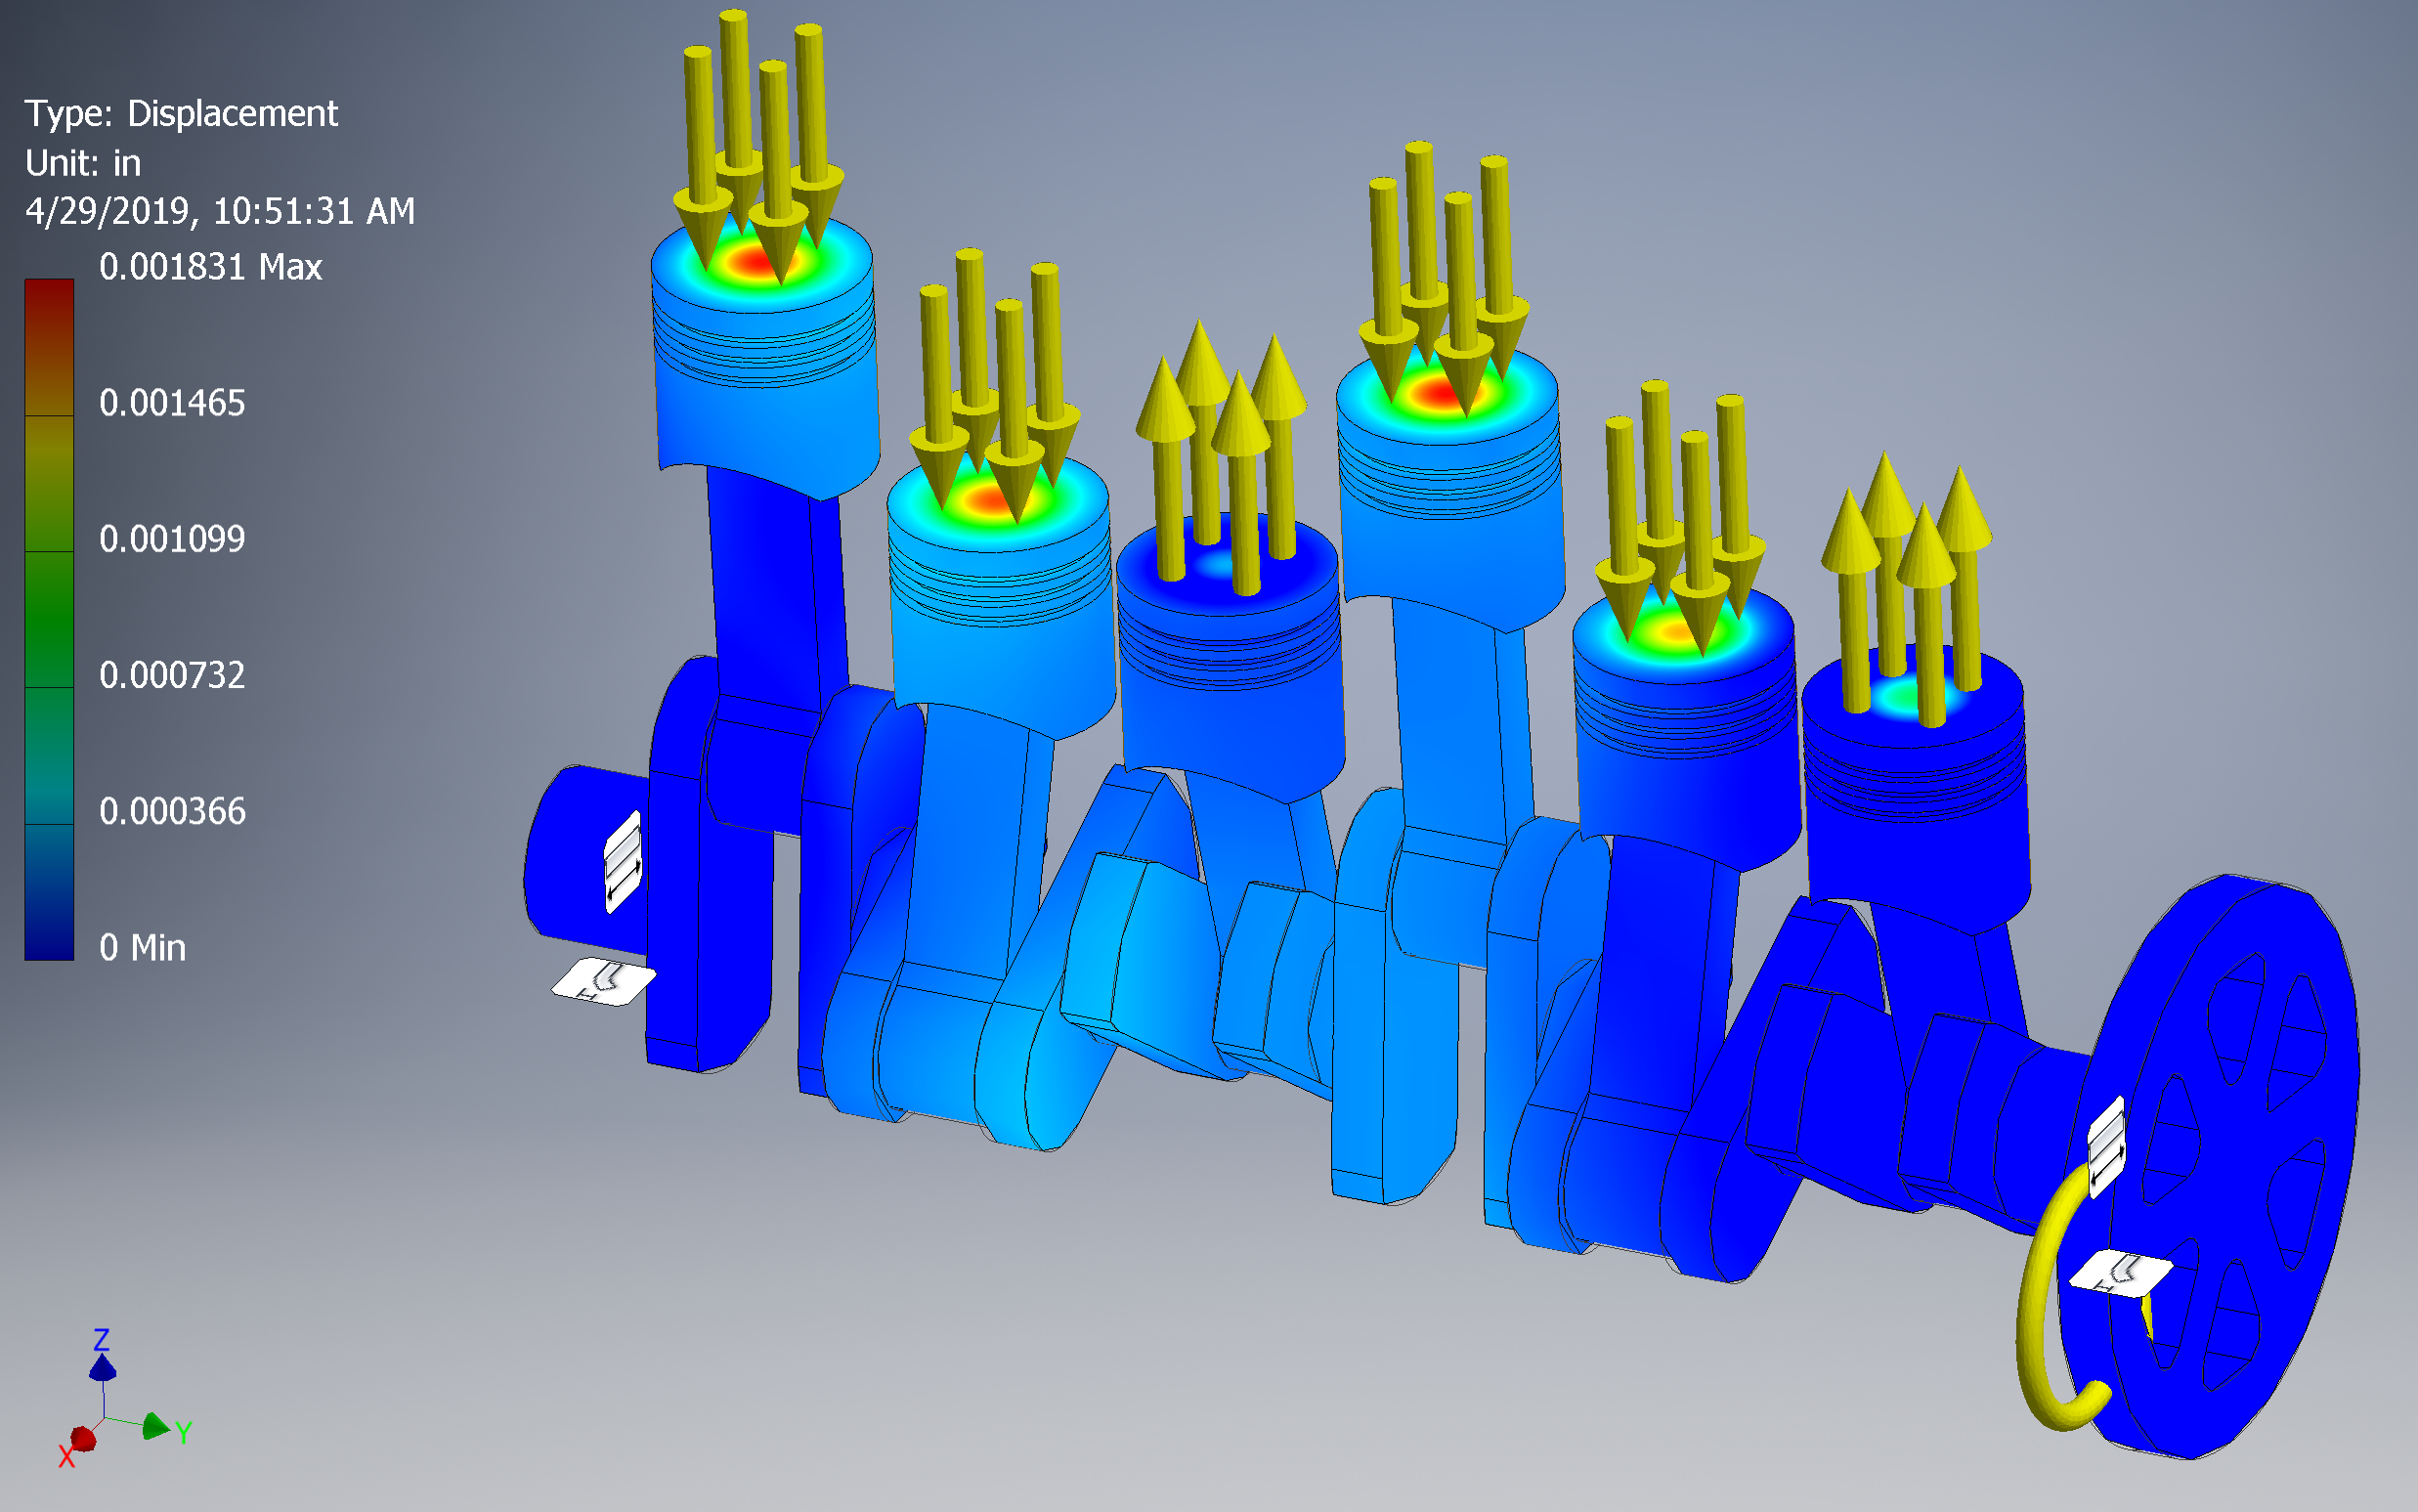
\includegraphics[width=\textwidth]{Displacement.png}
		\caption{Displacement Analysis performed in SolidWorks}
		\label{fig:diagram4}
	\end{figure}
Both of the figures suggest strong performance factors. Unfortunately, the dynamics of the systems were not accurately simulated. As such, the shaft stresses are too small.
\newpage
\section*{Conclusion}

\newpage
\section*{References}
Shigley, J. E., Mischke, C. R., Budynas, R. G., \& Shigley, J. E. (2006). \textit{Shigleys Mechanical Engineering Design} New York: McGraw-Hill Higher Education. \\
Keenan, J. H., Chao, J., \& Kaye, J. (1985). \textit{Gas Tables.} Taipei: Jwang Yuan Publishing.\\
Material properties were used from \textit{matweb.com}
\end{document}
